\chapter{Einleitung}
Ein neues System zur innerräumlichen Lokalisierung stellt das sogenannte iBeacon-Verfahren (z. Dt. Leuchtfeuer) dar. Die Vorteile dieses Systems gegenüber bisherigen Indoor-Lokalisierunglösungen sind zum einen die geringen Kosten, sowie die hohe Flexibilität/Autonomie der einzelnen Elemente. Denn viele andere Ansätze, wie z.B. die Indoor-Positionierung mit künstlichen Magnetfeldern \cite{Magnet}, die WLAN-basierte Ortung \citep{WLAN} oder andere hochfrequenz-basierte Entfernungsmessungen benötigen eine teure und aufwendige Infrastruktur, welche auch eine bauliche Änderung am Gebäude benötigen. Die Einfachheit der Anbringung der Beacons und die weitere Verbreitung des verwendeten Bluetooth-Protokolls auf mobilen Geräten sorgen für ein großes Einsatzspektrum und fördern dabei dessen Verbreitung. 


\section{Entwicklungsgeschichte}
Der Grundstein für die Beacon-Technologie legte die Firma Nokia im Jahre 2006. Damals entwickelte die Firma den neuen Standard \textit{Wibree} für die Funkübertragung,
\begin{wrapfigure}{r}{5.3cm}
\centering
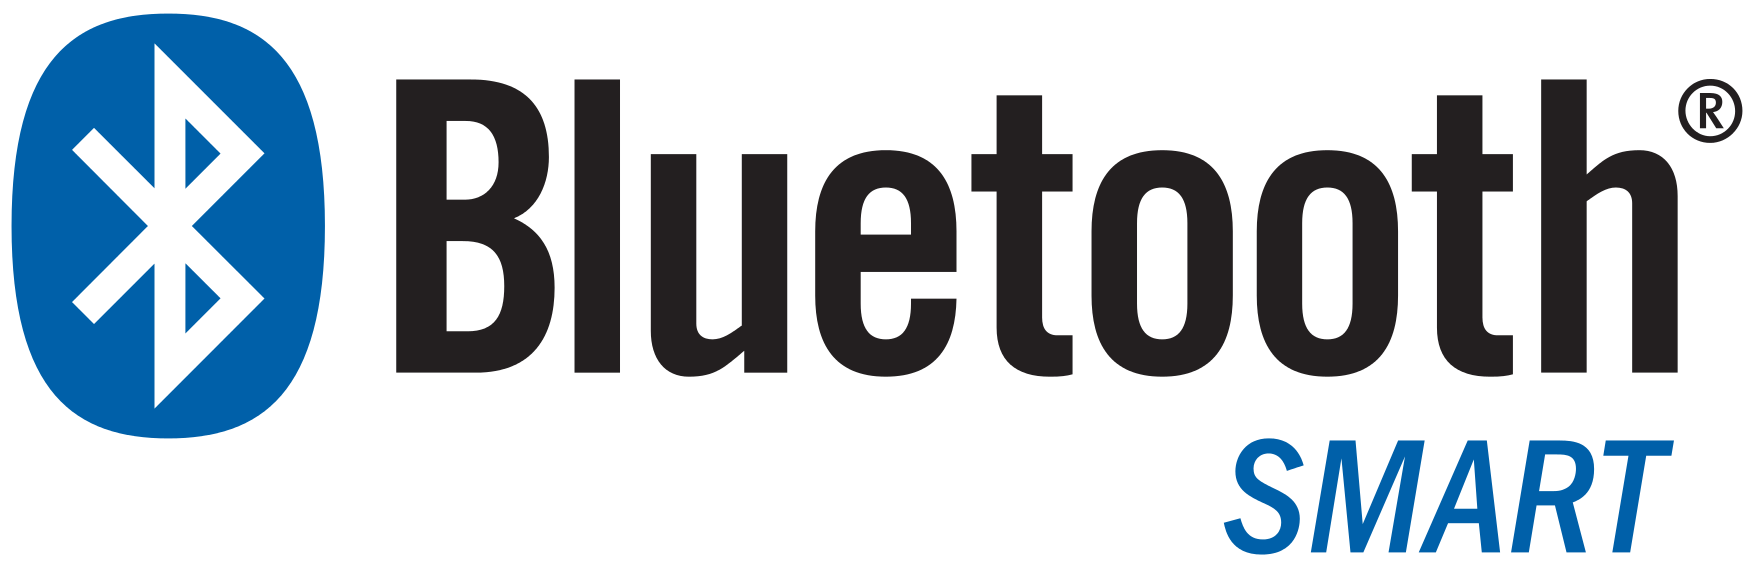
\includegraphics[scale=0.07]{Bilder/BLE.png} 
\caption{Offizielles Bluetooth Smart Logo \cite{BLElogo}}
\label{BLElogo}
\end{wrapfigure} der den alten Bluetooth-Standard ersetzen sollte. Mit der Neuentwicklung versprach man sich im Gegensatz zu Bluetooth einen geringeren Stromverbrauch und geringere Kosten, bei einem gleichbleibenden Kommunikationsbereich. Ab dem Jahr 2009 wurde der Bluetooth-Standard um Wibree ergänzt, unter dem Namen \textit{Bluetooth Low Energy (BLE)} darin aufgenommen \cite{Wib2BLE} und anschließend unter \textit{Bluetooth Smart} vermarktet.

\vspace{2\baselineskip}

\begin{wrapfigure}{l}{4cm}
\centering

\includegraphics[scale=0.5]{Bilder/iBeaconLogo.png} 
\caption{Offizielles iBeacon Logo \cite{iLogo}}
\label{iLogo}
\end{wrapfigure} Die Idee der Nutzung von Bluetooth Low Energy zur Indoor-Lokalisierung stammt dabei von der Firma Apple Inc. und wurde von ihr im Jahre 2013 auf der WWDC (Worldwide Developers Conference)\cite{Apple} unter dem Namen \textit{iBeacon} angekündigt. Obwohl zu dem Zeitpunkt noch kein fertiges Gerät zur Verfügung stand, wurde diese Technologie als Neuerung in Apples mobilen Betriebssystem iOS 7 vorgestellt. Jedoch verzichtet Apple seither auf die Produktion von iBeacons, was andere Unternehmen nutzen um selbst in den Markt einzusteigen. Deren Produkte unterstützen dabei zusätlich die mobilen Betriebssysteme Android ab Version 4.3 und Windows Phone 8. Somit wäre die Beacon-Technologie mittlerweile in über 99,5\% aller mobilen Geräte (Smartphones, Tablets, Smartwatches, etc.) weltweit nutzbar \cite{MobGerSt}.

\section{Aufbau und Funktionsweise von Beacons}
Die Grundbausteine eines Beacon sind ein Mikrocontroller, ein BLE-Sendemodul und eine Batterie. Anschaulich wird dies in Abbildung XXX, wo ein \textit{Estimote Beacon} der Firma Estimote Inc. in mehreren Schichten zu sehen ist. Die Estimote Beacons sind representativ für die Produkte der gesamten Branche, weswegen sie auch als Referenzprodukt für diese Arbeit dienen. 
\begin{wrapfigure}{r}{6cm}
\begin{flushright}
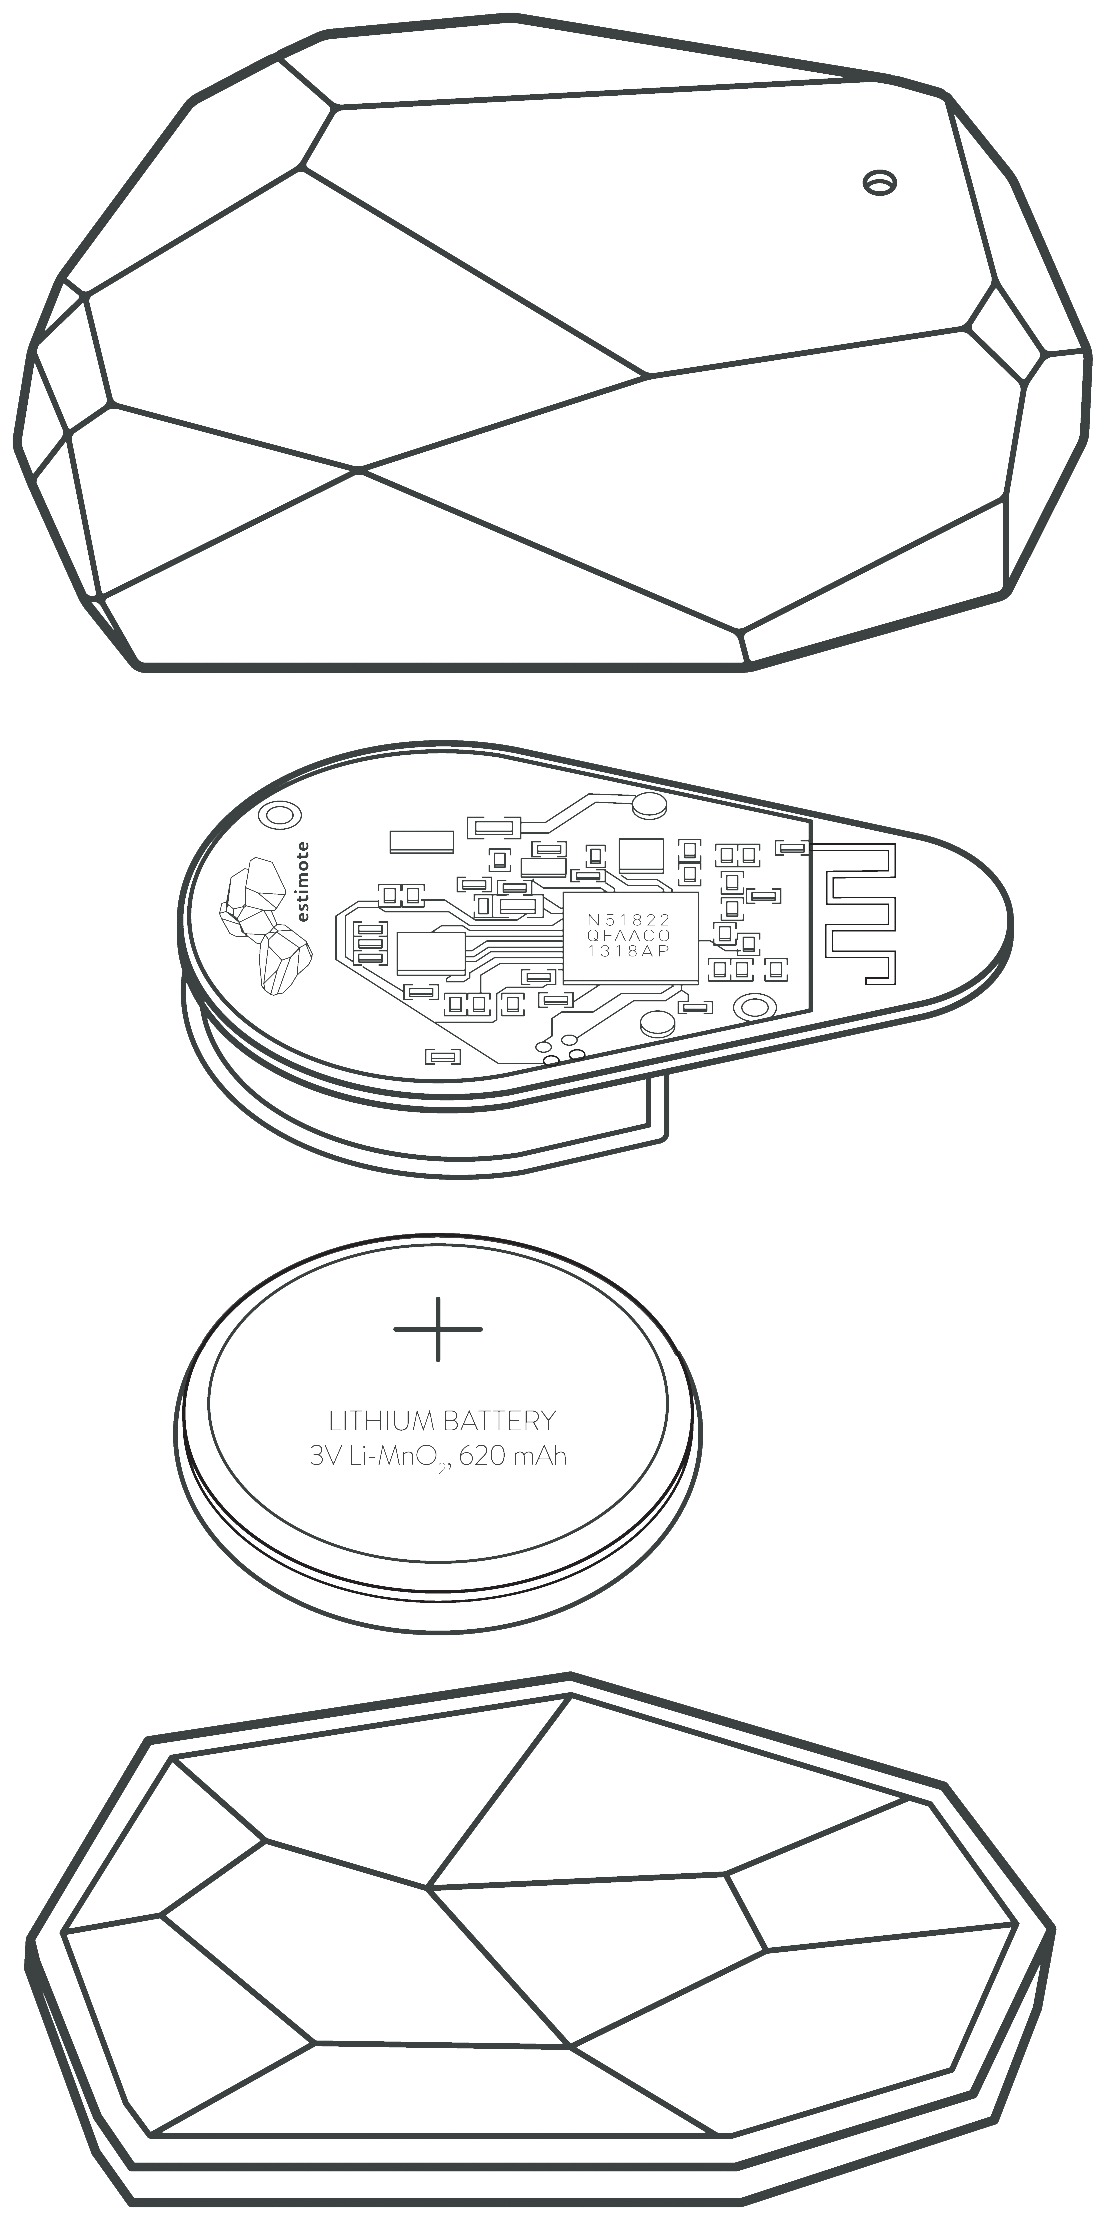
\includegraphics[scale=0.07]{Bilder/BeaconSchicht.png}
\caption{Explosionszeichnung Beacon \cite{BeaEx}}
\label{iLogo}
\begin{picture}(0,0)
\put(-150,177){Schutzhülle}
\put(-85,182){\line(1,0){25}}
\put(-150,137){Platine}
\put(-110,142){\line(1,0){50}}
\put(-150,100){Batterie}
\put(-100,105){\line(1,0){40}}
\put(-150,60){Silikonplatte}
\put(-80,65){\line(1,0){20}}
\end{picture}
\end{flushright}
\end{wrapfigure}

(Foto von einem nackten Beacon mit Erklärung, bzw. Linien einzeichnen und nummerieren (Antenne, Mikrocontroller, Batterie))

Die Beacons haben eine Sendeleistung von ... bis ... und senden in Intervallen von ... bis ... ms. Unidirektionale Übertragung. 

Dabei sendet ein beacon im Bluetooth Low Energy Protokoll  Zur Lokalisierung senden die Beacons drei Informationen:
\begin{itemize}
\item Identifikationsnummer
\item eingestellte Signalstärke
\item zusätzliche Angaben
\end{itemize}

(Bilder)

Änderbar sind die:
\begin{itemize}
\item Identifikationsnummer
\item eingestellte Signalstärke
\item Sendeintervall
\item zusätzliche Angaben
\end{itemize}

iBeacons sind kleine Bluetooth-Sender die im Raum plaziert werden und anhand des Verlustes der Signalstärke über die Distanz wird die Position relativ vom Empfänger zum Beacon berechnet. Die Strukturen in Gebäuden, wie Wände, Decken und Raumelemente, haben dabei einen negativen Einfluss auf die Signale und erschweren die Berechnung der Position. Es gilt nun ein Verfahren zu entwickeln, welches die Positionierung der iBeacons

Hier könnten theoretische Annahmen beschrieben und erklärt werden. Zum Beispiel ließe sich hier die Funktionsweise von iBeacons erklären, zusammen mit einer kleinen Einleitung in WLAN und Bluetooth (also welche Kanäle benutzt Bluetooth LE, sind die Beacons so schlau und suchen vor einer Signalsendung den Raum ab, ob gerade jemand anderes sendet und warten somit auf einen "freien" Raum). Desweiteren warum 2,4 Ghz als Frequenz beim Bluetooth LE-Format verwendet wird (Politik mit Vergabe der Sendefrequenzen, bei 2,4 Ghz ist die Eigenschwingung von Wasser, deswegen ist diese Frequenz frei, usw.).

Als Referenzprodukt für Beacons dient in dieser Arbeit das \textit{Estimote Beacon} von der Firma \textit{Estimote Inc.}. Als Auswahlkriterium diente zum einen die Verfügbarkeit des Produktes, sowei eine funktionierende SDK, um den Entwicklungsaufwand so gering wie möglich zu halten.
%\section{Verwendungsszenarien}
%Heute und morgen.
%
%Der Bedarf an einer innerräumlichen Ortung ist dort vorhanden, wo es für den Besucher schwer ist sich zu orientieren. Diese können sein: Flugplätze, Einkaufszentren und Messehallen. Das Ziel ist es nun den Besuchern dieser Einrichtungen ein ähnliches System bereit zu stellen, wie sie es von den Verkehrswegen her kennen. Es soll mithilfe mobiler Geräte (z.B. Smartphones) lokalisieren und gegebenenfalls durch das Gebäude navigieren möchte, wie er es von den Verkehrswegen her gewohnt ist.
%
%Denn in großen Gebieten, wie z.B. Einkaufshäuser, Lagerhallen und Flughäfen braucht man Hunderte von iBeacons, um die gesamte Fläche zu 100 Prozent abzudecken. Im Idealfall kann ich später in Matlab noch Gebiete einpflegen, an der die Karte nach Regionen aufgeteilt wird, in denen die Genauigkeit der Lokalisierung eingestellt werden kann. Damit ließe sich Robotergestützt ein Gebiet abfahren, in denen Vorschläge für die Positionierung von iBeacons anhand eines Optimierungsalgorithmusses generiert werden. Hierbei ließe sich wunderschön eine Pareto-Front bilden, die aus Anzahl von iBeacons und Genauigkeit pro Region Positionierungsvorschläge entwirft. Je nach Kundenwunsch. ROTER FADEN ZU MEINER ARBEIT1
%
%Hier kann angesprochen werden das wir ein adaptives Verfahren entwickeln wollen, denn viele bisherige Systeme bieten lediglich ein Landmarkenssystem oder ein Positionierungssystem. Mit den Beacons soll beides möglich sei und je nach Kundenwunsch anpassbar werden.
%
%\subsection{Landmarkensysteme}
%
%\subsection{Positionierungssysteme}
%
% 